\chapter{Aufz�hlungen und Tabellen}

Eine normale Punktliste:
\begin{itemize}
\item Lorem ipsum dolor sit amet, consectetuer adipiscing elit. Nulla ac ipsum a metus viverra tempor. 
\item Nunc sem. Nulla nec urna eu nibh vehicula convallis. Integer ac turpis. Donec mauris enim, dignissim quis, scelerisque ac, rhoncus id, sapien. 
\item Donec turpis felis, cursus in, varius vitae, mollis ac, lorem. Integer a dui sit amet eros nonummy aliquet. Donec egestas adipiscing tellus. Nulla iaculis. 
\item Aliquam erat volutpat. Curabitur posuere, eros vitae accumsan semper, risus erat viverra erat, eu vehicula mi leo at elit. Fusce luctus. Fusce vehicula pretium diam. Nunc sed arcu ut erat suscipit fermentum.
\end{itemize}

Eine nummerierte Liste:
\begin{enumerate}
\item Lorem ipsum dolor sit amet, consectetuer adipiscing elit. Nulla ac ipsum a metus viverra tempor. 
\item Nunc sem. Nulla nec urna eu nibh vehicula convallis. Integer ac turpis. Donec mauris enim, dignissim quis, scelerisque ac, rhoncus id, sapien. 
\item Donec turpis felis, cursus in, varius vitae, mollis ac, lorem. Integer a dui sit amet eros nonummy aliquet. Donec egestas adipiscing tellus. Nulla iaculis. 
\item Aliquam erat volutpat. Curabitur posuere, eros vitae accumsan semper, risus erat viverra erat, eu vehicula mi leo at elit. Fusce luctus. Fusce vehicula pretium diam. Nunc sed arcu ut erat suscipit fermentum.
\end{enumerate}

\section{Vom Autor verwendete Software}
\label{sec:Werkzeuge}
Im Folgenden werden die Programme vorgestellt, die der Autor zum Erstellen dieser Arbeit und vor allem zur Entwicklung der Webservices verwendet hat. Soweit es m�glich war, wurden Open-Source-Programme eingesetzt.

\begin{itemize}
\itemd{Microsoft Visio}{Die EPKs der BAP wurden mit Microsoft Visio erstellt. Der Autor hat zwar verschiedene Open-Source-Programme\footnote{Dia, OpenOffice Draw und die EPC Tools.} ausprobiert, mit denen EPKs erstellt werden k�nnten, die grafischen Ergebnisse waren aber nicht zufriedenstellend. Die Symbole von Visio sehen den "`originalen"' ARIS-Symbolen am �hnlichsten und k�nnen dar�ber hinaus mit zus�tzlichen Informationen wie Dauer und Kosten versehen werden.}
\itemd{PSPad}{F�r die Bearbeitung von verschiedenen (Text-)Dateien wurde der Texteditor PSPad verwendet. Mit diesem konnten \zB auch die regul�ren Ausdr�cke f�r die XML-Schemas entwickelt werden. Website: \url{http://www.pspad.com/}}
\itemd{Eclipse}{Sowohl der ActiveBPEL Designer als auch die EntireX Workbench sind Plugins f�r die IDE Eclipse. Auch zur Java- und PHP-Entwicklung wurde dieses Werkzeug verwendet. Website: \url{http://www.eclipse.org/}}
\itemd{XML Copy Editor}{F�r die Entwicklung der XML-Schemas und die Bearbeitung von XML-Dateien wurde der XML Copy Editor eingesetzt. Mit diesem k�nnen \ua XML-Dateien auf Wohlgeformtheit gepr�ft und gegen ihr Schema validiert werden. Website: \url{http://xml-copy-editor.sourceforge.net/}}
\itemd{soapUI}{
Mit soapUI k�nnen Webservices getestet werden, ohne einen Client zu programmieren. Die SOAP-Anfragen werden automatisch anhand der WSDL generiert und die Antworten k�nnen gegen die WSDL-Datei validiert werden. Website: \url{http://www.soapui.org/}}
\itemd{Ethereal}{
Die Netzwerkkommunikation beim Aufrufen der Webservices wurde mit Ethereal, einem umfangreichen Werkzeug zur Analyse des Netzwerkverkehrs, mitgeschnitten. Website: \url{http://www.ethereal.com/}}
\itemd{\LaTeX}{
Diese Arbeit wurde mit {\LaTeX} geschrieben. Als Distribution wurde MiKTeX verwendet und als Editor der LaTeX Editor. Websites: \url{http://miktex.org/}, \url{http://www.latexeditor.org/}}
\end{itemize}

\section{Elemente der Ereignisgesteuerten Prozesskette}

\begin{longtable}{|m{10cm}|m{3cm}|}
\caption{Elemente der Ereignisgesteuerten Prozesskette} \\
\hline
\label{tab:ElementeDerEreignisgesteuertenProzesskette}
\textbf{Element} & \textbf{Symbol}\\
\hline
\textbf{Funktion} 

Funktionen beschreiben T�tigkeiten, die im Verlauf des Gesch�ftsprozesses anfallen. Sie k�nnen von Mitarbeitern oder einem Informationssystem durchgef�hrt werden und ben�tigen evtl. Ressourcen, die ihnen zugewiesen werden. 

Beispiele: \textit{Auftrag anlegen}, \textit{Rechnung schreiben}, \textit{Konto abschlie�en} & 
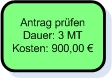
\includegraphics[width=3cm]{EPK-Funktion.jpg} \\
\hline
\textbf{Ereignis} 

Ereignisse sind betriebswirtschaftlich relevante Ereignisse, die den Gesch�ftsprozess in irgendeiner Weise steuern oder beeinflussen. Ereignisse sind immer Ausl�ser oder Ergebnisse von Funktionen. Ein Gesch�ftsprozess beginnt und endet stets mit einem Ereignis. 

Beispiele: \textit{Auftrag eingetroffen}, \textit{�berweisung get�tigt}, \textit{Rechnung erstellt} & 
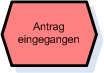
\includegraphics[width=3cm]{EPK-Ereignis.jpg} \\
\hline
\textbf{Operatoren} 

Operatoren steuern den Kontrollfluss eines Gesch�ftsprozesses. Sie machen \zB deutlich, dass eine Funktion mehrere Ereignisse ausl�st, oder zeigen alternative Vorgehensweisen an. Es gibt drei Operatoren (v.\,l.\,n.\,r.\,): UND, ODER und XODER (exklusives ODER). & 

\includegraphics[width=3cm]{EPK-Operatoren.jpg} \\
\hline
\textbf{Organisationseinheit} 

Organisationseinheiten werden Funktionen zugeordnet und beschreiben, wo die Funktionen ausgef�hrt werden bzw. wer sie ausf�hrt. Die Bezeichnung der Symbole enth�lt zus�tzlich zur Abteilung noch die Namen der Mitarbeiter.

Beispiele: \textit{Vertrieb}, \textit{Personal}, \textit{Produktion} & 
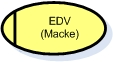
\includegraphics[width=3cm]{EPK-Organisationseinheit.jpg} \\
\hline
\textbf{Informationsobjekt} 

Auch Informationsobjekte werden Funktionen zugewiesen und beschreiben die von diesen ben�tigten oder erstellten Informationen. Dabei sind s�mtliche Formen von Informationen auf verschiedenen Datentr�gern m�glich und nicht etwa nur digitale Daten. Die Bezeichnung der Symbole enth�lt zus�tzlich das Informationssystem, aus dem die Informationen stammen.

Beispiele: \textit{Kundendatenbank}, \textit{Versicherungsantrag}, \textit{Rechnung} & 
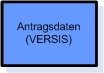
\includegraphics[width=3cm]{EPK-Informationen.jpg} \\
\hline
\textbf{Prozesswegweiser}

Mit Prozesswegweisern werden Prozesse, die in anderen EPKs beschrieben sind, referenziert. So k�nnen \zB un�bersichtliche Prozesse in Teilprozesse gegliedert und h�ufig verwendete Prozesse an zentraler Stelle modelliert werden. Prozesswegweiser stehen in einer EPK immer anstelle von Funktionen. & 
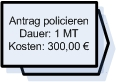
\includegraphics[width=3cm]{EPK-Prozesspfad.jpg} \\
\hline
\end{longtable}
